\documentclass[tikz]{standalone}
% A BREEZE IN THE MEADOW -- original Monet-inspired impressionist interpretation.
% Retains the boy, tree, kite, and the continuous hand-to-kite string.
% All marks are editable TikZ vectors; no external image, font, or data required.
% Fixed random seed makes the broken-color brushwork reproducible.
% Compile: pdflatex -interaction=nonstopmode -halt-on-error -output-directory=tmp mweM.tex
\definecolor{canvas}{HTML}{F2EDDF}
\definecolor{sky}{HTML}{C5DCE5}
\definecolor{skyblue}{HTML}{AFCEDA}
\definecolor{skywhite}{HTML}{E6E9DF}
\definecolor{cream}{HTML}{F7EAD0}
\definecolor{cloudrose}{HTML}{DFD7D5}
\definecolor{haze}{HTML}{B4C6C6}
\definecolor{farblue}{HTML}{91AEB6}
\definecolor{farwillow}{HTML}{A8BBA2}
\definecolor{grass}{HTML}{9EB577}
\definecolor{grassgold}{HTML}{C3C687}
\definecolor{sunleaf}{HTML}{D4D396}
\definecolor{lemon}{HTML}{E7DDA0}
\definecolor{leaf}{HTML}{8DA56A}
\definecolor{leafgreen}{HTML}{769665}
\definecolor{leafblue}{HTML}{65887E}
\definecolor{leafdeep}{HTML}{55766F}
\definecolor{shadow}{HTML}{7C88A0}
\definecolor{lavender}{HTML}{A4A1B4}
\definecolor{lilac}{HTML}{BBB2C1}
\definecolor{earth}{HTML}{ADAA82}
\definecolor{bark}{HTML}{AC9B84}
\definecolor{barklight}{HTML}{D2BE98}
\definecolor{barkshade}{HTML}{7B8491}
\definecolor{skin}{HTML}{E4BC98}
\definecolor{skinlight}{HTML}{F1D3AF}
\definecolor{skinshade}{HTML}{BEA498}
\definecolor{hair}{HTML}{77736D}
\definecolor{hairlight}{HTML}{A69D83}
\definecolor{shirt}{HTML}{EFE8CC}
\definecolor{shirtshade}{HTML}{B8C8CB}
\definecolor{red}{HTML}{BA7B71}
\definecolor{redlight}{HTML}{D69781}
\definecolor{redshade}{HTML}{967E8B}
\definecolor{shoe}{HTML}{698697}
\definecolor{rose}{HTML}{D6A3AE}
\definecolor{kiteblue}{HTML}{91B9CB}
\definecolor{line}{HTML}{777D85}

% Broken-color scumble: marks per pigment, box x/y/w/h, brush w/h, palette.
% Separate marks rather than a raster texture keep the output fully vector.
\newcommand{\Scumble}[8]{%
  \foreach \pigment in {#8}{%
    \foreach \stroke in {1,...,#1}{%
      \pgfmathsetmacro{\px}{#2+rnd*(#4)}%
      \pgfmathsetmacro{\py}{#3+rnd*(#5)}%
      \pgfmathsetmacro{\bw}{(#6)*(0.55+0.9*rnd)}%
      \pgfmathsetmacro{\bh}{(#7)*(0.55+0.9*rnd)}%
      \pgfmathsetmacro{\tilt}{-24+48*rnd}%
      \path[fill=\pigment,opacity=.52,shift={(\px,\py)},rotate=\tilt]
        (0,0) .. controls (.25*\bw,-.35*\bh) and (.8*\bw,-.2*\bh) .. (\bw,0)
        -- (.88*\bw,.64*\bh)
        .. controls (.58*\bw,1.05*\bh) and (.2*\bw,.8*\bh) .. (-.08*\bw,.62*\bh)
        -- cycle;
    }%
  }%
}

% Irregular translucent underpainting and overlapping curved dabs avoid circular edges.
\newcommand{\LeafCluster}[5]{%
  \path[fill=#5,opacity=.30] plot[smooth cycle,tension=.6] coordinates {
    (#1-.94*#3,#2-.18*#4) (#1-.69*#3,#2-.68*#4)
    (#1-.35*#3,#2-.81*#4) (#1+.03*#3,#2-.97*#4)
    (#1+.46*#3,#2-.73*#4) (#1+.82*#3,#2-.48*#4)
    (#1+.93*#3,#2+.07*#4) (#1+.72*#3,#2+.52*#4)
    (#1+.32*#3,#2+.81*#4) (#1-.11*#3,#2+.91*#4)
    (#1-.56*#3,#2+.66*#4) (#1-.87*#3,#2+.31*#4)};
  \foreach \pigment in {leafgreen,leafblue,leaf,grassgold,sunleaf}{%
    \foreach \stroke in {1,...,65}{%
      \pgfmathsetmacro{\angle}{360*rnd}%
      \pgfmathsetmacro{\radius}{sqrt(rnd)}%
      \pgfmathsetmacro{\px}{#1+\radius*(#3)*cos(\angle)}%
      \pgfmathsetmacro{\py}{#2+\radius*(#4)*sin(\angle)}%
      \pgfmathsetmacro{\bw}{4+9*rnd}%
      \pgfmathsetmacro{\bh}{2+5*rnd}%
      \pgfmathsetmacro{\tilt}{-50+100*rnd}%
      \path[fill=\pigment,opacity=.64,shift={(\px,\py)},rotate=\tilt]
        (0,0) .. controls (.3*\bw,-.35*\bh) and (.8*\bw,-.2*\bh) .. (\bw,.2*\bh)
        -- (.8*\bw,.7*\bh)
        .. controls (.4*\bw,1.1*\bh) and (.1*\bw,.8*\bh) .. (0,0) -- cycle;
    }%
  }%
}
\begin{document}
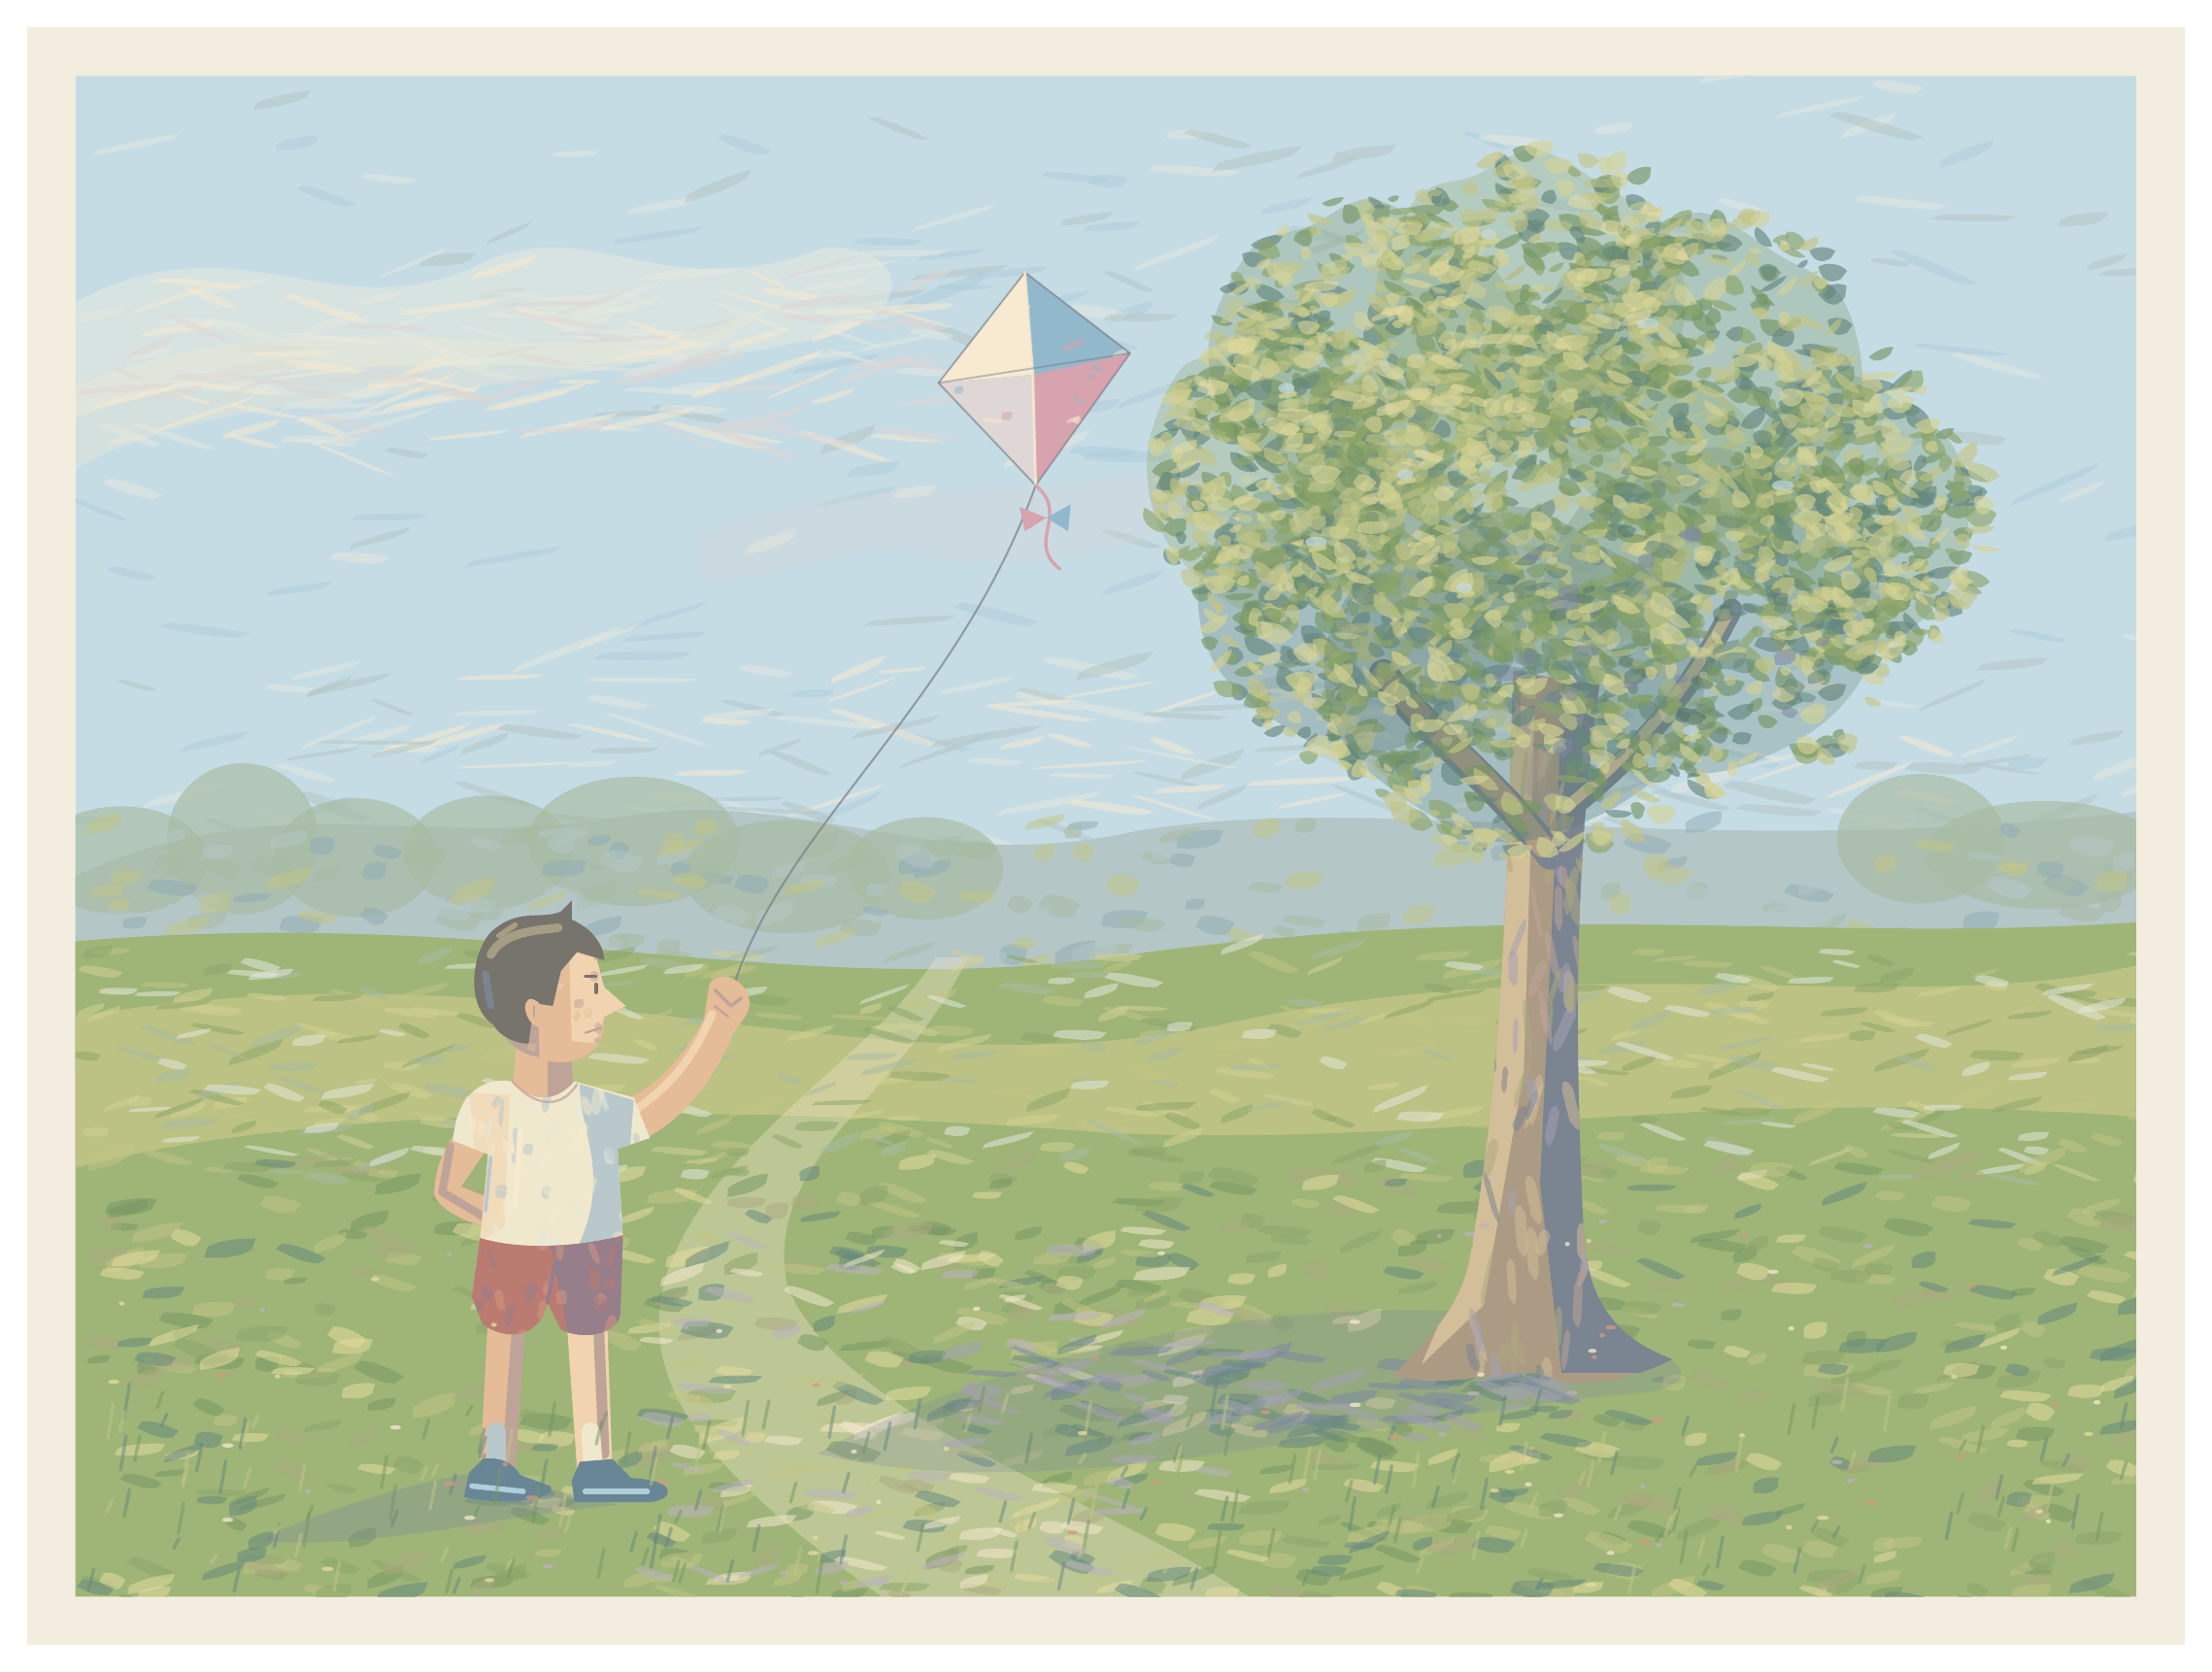
\begin{tikzpicture}[x=1bp,y=-1bp,line cap=round,line join=round]
  \pgfmathsetseed{187406}
  \path[use as bounding box] (0,0) rectangle (800,600);
  \fill[canvas] (0,0) rectangle (800,600);
  \begin{scope}
    \clip (18,18) rectangle (782,582);
    % 1. Sky: cool luminous underpaint, warm drifting cloud veils.
    \fill[sky] (18,18) rectangle (782,365);
    \Scumble{80}{15}{18}{775}{325}{24}{3}{skyblue,skywhite,haze}
    \path[fill=skywhite,opacity=.55] (18,102)
      .. controls (80,69) and (113,114) .. (168,88)
      .. controls (209,68) and (236,105) .. (295,82)
      .. controls (329,80) and (333,111) .. (285,117)
      .. controls (205,136) and (111,111) .. (18,145) -- cycle;
    \path[fill=cream,opacity=.3] (18,133)
      .. controls (124,91) and (198,139) .. (279,102)
      .. controls (223,147) and (88,123) .. (18,164) -- cycle;
    \path[fill=cloudrose,opacity=.25] (249,189)
      .. controls (313,159) and (386,181) .. (431,159)
      .. controls (464,178) and (397,205) .. (337,197)
      .. controls (306,187) and (285,207) .. (249,205) -- cycle;
    \Scumble{50}{20}{90}{310}{65}{27}{2}{skywhite,cream,cloudrose}
    \Scumble{35}{80}{237}{650}{57}{29}{2}{skywhite,cream,haze}

    % 2. A low, hazy tree line; no hard horizon stroke.
    \path[fill=haze] (18,315)
      .. controls (92,280) and (148,306) .. (220,293)
      .. controls (288,281) and (333,316) .. (412,298)
      .. controls (506,283) and (613,310) .. (782,291)
      -- (782,387) -- (18,387) -- cycle;
    \foreach \x/\y/\rx/\ry in {35/309/32/20,80/301/28/28,122/308/30/22,
      171/306/31/21,225/302/39/24,282/315/38/21,333/312/29/19,
      702/301/31/24,748/307/44/20}{
      \fill[farwillow,opacity=.65] (\x,\y) ellipse[x radius=\rx bp,y radius=\ry bp];
    }
    \Scumble{55}{20}{295}{760}{55}{12}{5}{farblue,farwillow,haze,grassgold}
    \fill[grass] (18,339)
      .. controls (186,325) and (285,364) .. (416,343)
      .. controls (571,323) and (662,340) .. (782,332)
      -- (782,582) -- (18,582) -- cycle;
    \path[fill=grassgold,opacity=.8] (18,367)
      .. controls (198,337) and (308,399) .. (447,369)
      .. controls (582,340) and (697,368) .. (782,348)
      -- (782,404) .. controls (614,392) and (531,416) .. (400,410)
      .. controls (234,397) and (97,402) .. (18,423) -- cycle;
    % A pale diagonal track leads toward the raised hand and the kite.
    \path[fill=cream,opacity=.34] (349,345)
      .. controls (324,397) and (272,420) .. (282,467)
      .. controls (302,516) and (398,545) .. (453,582)
      -- (317,582) .. controls (254,537) and (225,504) .. (237,463)
      .. controls (254,413) and (313,383) .. (337,345) -- cycle;
    \Scumble{85}{18}{342}{764}{84}{15}{2.5}{grassgold,sunleaf,leaf,farwillow,skywhite}
    \Scumble{115}{18}{420}{764}{162}{13}{4}{leafgreen,grassgold,leaf,earth,lemon,leafblue}
    \Scumble{45}{225}{445}{210}{135}{14}{3}{cream,grassgold,lilac}

    % Tree shadow: colored reflected light, never a black cast shadow.
    \path[fill=shadow,opacity=.25] (542,477)
      .. controls (458,470) and (359,493) .. (293,529)
      .. controls (383,551) and (503,514) .. (603,506)
      .. controls (636,498) and (584,480) .. (542,477) -- cycle;
    \Scumble{30}{331}{489}{239}{33}{16}{3}{shadow,leafblue,lavender}

    % 3. Trunk and branches: violet shadow, ochre reflected light, broken edges.
    \def\Trunk{(551,239)
      .. controls (549,302) and (548,384) .. (535,456)
      .. controls (531,479) and (514,490) .. (507,500)
      .. controls (532,507) and (551,493) .. (568,502)
      .. controls (579,505) and (599,500) .. (610,494)
      .. controls (583,484) and (578,465) .. (577,444)
      .. controls (573,359) and (575,301) .. (583,244) -- cycle}
    \path[fill=bark] \Trunk;
    \begin{scope}
      \clip \Trunk;
      \path[fill=barkshade] (570,232) -- (590,229) -- (581,444)
        -- (613,499) -- (569,499) -- (561,429) -- cycle;
      \path[fill=barklight] (544,249) -- (559,253) -- (555,387)
        -- (540,474) -- (517,496) -- (536,452) -- cycle;
      \Scumble{26}{532}{246}{57}{253}{3}{14}{barklight,barkshade,skinshade,lavender,earth}
    \end{scope}
    \draw[draw=barkshade,line width=11bp] (565,307)
      .. controls (543,278) and (520,263) .. (503,240);
    \draw[draw=bark,line width=8bp] (562,304)
      .. controls (543,277) and (522,263) .. (503,240);
    \draw[draw=barkshade,line width=8bp] (573,289)
      .. controls (604,264) and (620,240) .. (632,216);
    \draw[draw=barklight,line width=4bp] (571,289)
      .. controls (603,263) and (620,238) .. (631,217);

    % 4. Crown: overlapping masses with irregular leaf strokes and sky holes.
    \LeafCluster{496}{216}{65}{59}{leafdeep}
    \LeafCluster{552}{242}{75}{66}{leafdeep}
    \LeafCluster{625}{218}{67}{64}{leafblue}
    \LeafCluster{677}{183}{46}{55}{leafgreen}
    \LeafCluster{458}{166}{45}{56}{leaf}
    \LeafCluster{497}{125}{62}{63}{leafgreen}
    \LeafCluster{558}{103}{61}{59}{leaf}
    \LeafCluster{619}{132}{66}{65}{leafgreen}
    \LeafCluster{559}{175}{94}{66}{leaf}
    % Warm illumination is concentrated on upper-left planes, not everywhere.
    \begin{scope}
      \clip (493,139) ellipse[x radius=72bp,y radius=56bp];
      \Scumble{32}{424}{85}{135}{110}{10}{4}{sunleaf,lemon,grassgold}
    \end{scope}
    \begin{scope}
      \clip (559,103) ellipse[x radius=60bp,y radius=54bp];
      \Scumble{26}{500}{48}{120}{103}{9}{4}{sunleaf,lemon,grassgold}
    \end{scope}
    \begin{scope}
      \clip (605,230) ellipse[x radius=69bp,y radius=49bp];
      \Scumble{24}{536}{183}{138}{98}{8}{4}{leafdeep,leafblue,shadow}
    \end{scope}
    \foreach \x/\y/\r in {478/191/4,511/166/3,542/77/3,601/110/4,
      651/170/4,533/208/3,576/147/4,617/261/3,467/134/3}{
      \fill[sky,opacity=.66] (\x,\y) ellipse[x radius=\r bp,y radius=2bp];
      \draw[draw=sunleaf,opacity=.75,line width=1.8bp] (\x-2,\y+3) -- (\x+3,\y+2);
    }

    % 5. Kite: small high-chroma accents against open sky, no black perimeter.
    \coordinate (kite-knot) at (374,170);
    \coordinate (hand) at (260,363);
    \draw[draw=line,opacity=.68,line width=.75bp] (hand)
      .. controls (275,301) and (344,254) .. (kite-knot);
    \def\Kite{(370,91) -- (409,121) -- (374,170) -- (338,132) -- cycle}
    \path[fill=rose] \Kite;
    \fill[cream] (370,91) -- (373,129) -- (338,132) -- cycle;
    \fill[kiteblue] (370,91) -- (409,121) -- (373,129) -- cycle;
    \fill[cloudrose] (338,132) -- (373,129) -- (374,170) -- cycle;
    \begin{scope}
      \clip \Kite;
      \Scumble{8}{338}{93}{71}{75}{6}{2}{cream,rose,kiteblue}
    \end{scope}
    \draw[draw=line,opacity=.6,line width=.7bp] \Kite;
    \draw[draw=cream,opacity=.85,line width=1bp] (370,91) -- (373,129) -- (374,170);
    \draw[draw=line,opacity=.45,line width=.7bp] (338,132) -- (409,121);
    \draw[draw=rose,line width=1.2bp] (374,170)
      .. controls (387,181) and (370,191) .. (383,201);
    \path[fill=rose] (378,182) -- (368,178) -- (370,187) -- cycle;
    \path[fill=kiteblue] (378,182) -- (387,177) -- (386,187) -- cycle;

    % 6. Boy: readable gesture and anatomy, with lost-and-found colored edges.
    \path[fill=shadow,opacity=.32] (167,536)
      .. controls (145,539) and (109,550) .. (86,561)
      .. controls (122,566) and (181,551) .. (219,548) -- cycle;
    % Legs and shoes.
    \path[fill=skin] (171,477) -- (184,479) -- (181,532)
      -- (168,536) -- cycle;
    \path[fill=skinshade] (180,480) -- (185,480) -- (181,534) -- (176,533) -- cycle;
    \path[fill=skinlight] (200,478) -- (215,476) -- (217,533)
      -- (204,535) -- cycle;
    \draw[draw=skinshade,line width=4bp] (212,483) -- (214,529);
    \draw[draw=shirtshade,line width=7bp] (174,521) -- (174,533);
    \draw[draw=shirt,line width=7bp] (209,521) -- (210,534);
    \path[fill=shoe] (169,531) .. controls (175,530) and (180,532) .. (183,537)
      -- (194,541) .. controls (198,547) and (172,548) .. (162,545)
      -- (164,536) -- cycle;
    \path[fill=shoe] (205,532) -- (217,531) -- (224,538)
      .. controls (242,539) and (240,546) .. (231,547)
      -- (203,547) -- (202,539) -- cycle;
    \draw[draw=skyblue,line width=2bp] (165,541) -- (184,543);
    \draw[draw=skyblue,line width=2bp] (207,543) -- (230,543);

    % Near arm folded by the waist; far arm reaches up to hold the string.
    \path[fill=skin] (165,405)
      .. controls (156,410) and (151,423) .. (151,433)
      .. controls (153,439) and (166,445) .. (173,445)
      -- (176,436) -- (161,430) -- (174,411) -- cycle;
    \draw[draw=skinshade,line width=3bp] (157,415) -- (154,432) -- (169,441);
    \path[fill=skin] (217,399)
      .. controls (232,396) and (244,381) .. (251,368)
      -- (253,355) .. controls (256,350) and (264,352) .. (267,358)
      .. controls (270,365) and (265,368) .. (262,373)
      .. controls (253,395) and (238,410) .. (224,414) -- cycle;
    \draw[draw=skinlight,line width=3bp] (225,402)
      .. controls (241,391) and (248,380) .. (254,366);
    \draw[draw=skinshade,line width=1.2bp] (255,357) -- (261,363) -- (265,360);
    \draw[draw=skinshade,line width=.8bp] (255,363) -- (260,367);

    % Neck, softly lit face and hair.
    \path[fill=skin] (182,373) -- (201,375) -- (203,396)
      .. controls (196,404) and (185,401) .. (180,394) -- cycle;
    \fill[skinshade] (193,378) -- (201,375) -- (203,396) -- (193,398) -- cycle;
    \def\Shirt{(180,391)
      .. controls (167,389) and (159,398) .. (158,413)
      -- (171,418) -- (168,450)
      .. controls (183,456) and (207,454) .. (221,449)
      -- (219,416) -- (231,412) -- (225,397) -- (203,391)
      .. controls (196,399) and (187,399) .. (180,391) -- cycle}
    \path[fill=shirt] \Shirt;
    \begin{scope}
      \clip \Shirt;
      \path[fill=shirtshade] (205,392) -- (225,398) -- (221,449)
        -- (204,453) .. controls (217,425) and (205,411) .. (205,392);
      \fill[skinlight,opacity=.6] (164,395) -- (179,396) -- (177,445) -- (169,450) -- cycle;
      \Scumble{13}{159}{394}{70}{58}{3}{7}{cream,skywhite,shirtshade,shirt}
    \end{scope}
    \draw[draw=skinshade,opacity=.7,line width=.9bp] (180,391)
      .. controls (190,402) and (199,400) .. (204,392);
    \draw[draw=shirtshade,line width=1.3bp] (172,419) -- (170,439);
    \draw[draw=cream,line width=2bp] (183,409) -- (181,437);

    \def\Shorts{(168,449)
      .. controls (184,454) and (207,452) .. (221,448)
      -- (220,477) .. controls (219,485) and (206,487) .. (198,483)
      -- (193,473) .. controls (190,487) and (177,487) .. (169,481)
      -- (165,471) -- cycle}
    \path[fill=red] \Shorts;
    \begin{scope}
      \clip \Shorts;
      \fill[redshade] (194,451) -- (222,449) -- (222,485) -- (201,486) -- cycle;
      \Scumble{12}{165}{450}{58}{36}{3}{6}{redlight,red,redshade}
    \end{scope}
    \draw[draw=redshade,line width=1.5bp] (193,473) -- (196,458);

    \def\Face{(173,347)
      .. controls (178,331) and (202,331) .. (211,344)
      -- (214,356) -- (222,363) -- (214,367)
      .. controls (215,382) and (201,387) .. (189,382)
      .. controls (176,379) and (169,365) .. (173,347) -- cycle}
    \path[fill=skin] \Face;
    \begin{scope}
      \clip \Face;
      \fill[skinshade] (172,340) -- (189,341) -- (190,382) -- (171,378) -- cycle;
      \fill[skinlight] (201,343) -- (211,345) -- (214,356)
        -- (222,363) -- (214,367) -- (211,377) -- (202,376) -- cycle;
      \Scumble{7}{174}{341}{40}{39}{3}{3}{skin,skinlight,skinshade}
    \end{scope}
    \path[fill=hair] (173,370)
      .. controls (161,362) and (166,339) .. (174,334)
      .. controls (183,327) and (191,331) .. (198,328)
      -- (202,324) -- (202,331)
      .. controls (209,334) and (214,340) .. (214,346)
      -- (204,343) -- (198,350) -- (195,363) -- (188,362)
      -- (186,377) .. controls (181,377) and (175,374) .. (173,370) -- cycle;
    \draw[draw=hairlight,line width=3.2bp] (172,344)
      .. controls (177,335) and (190,335) .. (197,334);
    \draw[draw=barkshade,line width=2.6bp] (170,351) -- (172,363);
    \draw[draw=hairlight,line width=2bp] (175,337) -- (181,333);
    \path[fill=skin] (190,362)
      .. controls (183,356) and (183,369) .. (190,371) -- cycle;
    \draw[draw=skinshade,line width=.8bp] (188,363) -- (188,367);
    \draw[draw=hair,line width=1.1bp] (207,352) -- (211,352);
    \draw[draw=hair,line width=1.3bp] (211,355) -- (211,358);
    \draw[draw=skinshade,line width=.8bp] (213,371) -- (207,373);

    % 7. Foreground: flowers and grass partly dissolve the feet into the meadow.
    \foreach \pigment in {leafgreen,leafblue,grassgold}{
      \foreach \stroke in {1,...,65}{
        \pgfmathsetmacro{\px}{20+760*rnd}
        \pgfmathsetmacro{\py}{512+70*rnd}
        \pgfmathsetmacro{\height}{3+10*rnd}
        \draw[draw=\pigment,opacity=.5,line width=1.2bp]
          (\px,\py) -- (\px+2,\py-\height);
      }
    }
    \foreach \pigment in {cream,lemon,lilac,redlight}{
      \foreach \flower in {1,...,22}{
        \pgfmathsetmacro{\px}{24+748*rnd}
        \pgfmathsetmacro{\py}{442+138*rnd}
        \pgfmathsetmacro{\size}{.8+1.6*rnd}
        \fill[\pigment,opacity=.75] (\px,\py)
          ellipse[x radius=\size bp,y radius=.8bp];
      }
    }
    % No signature, labels, dimensions, or raster overlays.
  \end{scope}
\end{tikzpicture}
\end{document}
